% ==============================================================================
% Springer Nature (sn-jnl) LaTeX Template for Information Systems Frontiers (ISF)
% Single-Column Format 
% ==============================================================================

\documentclass[sn-mathphys,Numbered]{sn-jnl}
% The 'twocolumn' option has been removed for single-column formatting.

\usepackage{graphicx}
\usepackage{multirow}
\usepackage{amsmath,amssymb,amsfonts}
\usepackage{amsthm}
\usepackage{mathrsfs}
\usepackage[title]{appendix}
\usepackage{xcolor}
\usepackage{textcomp}
\usepackage{manyfoot}
\usepackage{booktabs}
\usepackage{algorithm}
\usepackage{algorithmicx}
\usepackage{algpseudocode}
\usepackage{listings}
\usepackage{cuted} % For wide equations if needed
\usepackage{float} % Required to force algorithm placement with [H]

\theoremstyle{thmstyleone}
\newtheorem{theorem}{Theorem}
\newtheorem{proposition}[theorem]{Proposition}
\theoremstyle{thmstyletwo}
\newtheorem{example}{Example}
\newtheorem{remark}{Remark}
\theoremstyle{thmstylethree}
\newtheorem{definition}{Definition}

\raggedbottom

\begin{document}

\title[Neuro-Symbolic Disentangled Representations]{Streaming-Resilient Multimodal Emotion Recognition via Neuro-Symbolic Disentanglement}

% ==== AUTHORS HIDDEN FOR DOUBLE-BLIND REVIEW ====
% \author*[1]{\fnm{First Name 1} \sur{Surname 1}}\email{corresponding.author@email.com}
% \author[2]{\fnm{First Name 2} \sur{Surname 2}}\email{author2@email.com}
% \affil*[1]{\orgdiv{Your Department or Lab}, \orgname{Your University or Institute}...}
% \affil[2]{\orgdiv{Second Department or Lab}, \orgname{Second University or Institute}...}

\abstract{
Deploying Multimodal Emotion Recognition in real-world Information Systems is severely bottlenecked by environmental noise and hardware failures during live streaming.However, existing models fail catastrophically because they project raw modalities into entangled semantic spaces and rely on computationally massive, latency-inducing generative frameworks to hallucinate corrupted sensor data. To address these critical gaps, we propose the Dynamic Relational Context Fusion Network (DRCFNet), a novel Streaming Architecture that utilizes a Dual-Thread shadow paradigm and Disentangled Representations via dynamic gating---regularized by a Neuro-Symbolic AI logic graph---to separate modality-specific noise from shared semantics. We evaluated our approach on the benchmark CMU-MOSI and CMU-MOSEI datasets using a zero-latency predictive entropy governance layer. Extensive experiments demonstrate that DRCFNet achieves state-of-the-art predictive performance, securing highly robust F1-scores of 84.5\% on CMU-MOSI and 85.6\% on CMU-MOSEI while operating under a strict 15.8 ms latency constraint. Ultimately, this research provides a highly robust, explainable framework for deploying resilient affective agents in critical edge-based enterprise environments.
}

\keywords{Multimodal Emotion Recognition, Information Systems, Disentangled Representations, Neuro-Symbolic AI, Streaming Architecture}

\maketitle

% ==========================================
% SECTION 1: INTRODUCTION  (humanized prose; citations, numbers, and RQ statements unchanged)
% ==========================================
\section{Introduction}\label{sec1}
Information Systems (IS) have moved well beyond their origins as static repositories for data processing; today they are expected to be interactive and, increasingly, intelligent. Much of this shift sits within Human-Computer Interaction (HCI), where systems are now asked not only to process input but to perceive, interpret, and respond to human emotion \cite{picard2003affective, zeng2008survey, poria2017review}. The research area concerned with this capability, Affective Computing, has become foundational to how modern intelligent systems are designed. The market reflects that momentum: the global affective computing market was valued at roughly \$60 billion in 2023 and is projected to grow at a CAGR above 25\% through the 2030s. Two application areas account for much of the demand. The first is telehealth, where emotion-aware models are increasingly used for remote patient monitoring; the second is customer relationship management (CRM), where real-time emotional signals are used to tailor interactions. In both settings, Multimodal Emotion Recognition (MER)---the fusion of visual, acoustic, and textual streams---is what lets an agent respond in a way that feels context-aware rather than scripted \cite{poria2019emotion}.

Deep learning has driven real progress in MER \cite{gu2023comprehensive}, yet moving these models out of controlled laboratory conditions and into everyday Information Systems exposes a problem the algorithms themselves do not solve: hardware fails and signal quality degrades during live streaming. The cost is not marginal. Empirical work has reported accuracy drops of more than 40\% when models trained on curated datasets are deployed in noisy conditions, with ambient acoustic distortion or visual occlusion. The scenarios are mundane---a microphone cuts out mid-sentence, or a webcam feed blurs because bandwidth dropped---but most current architectures have no sensible fallback when a live stream is corrupted. The alternative they tend to offer is worse: large generative models that hallucinate the missing features at the cost of latency \cite{zhao2023missing}. This gap, between models that work offline and models that hold up under a real latency budget, motivates our first research question: \textit{RQ1 (Streaming Governance): Can intelligent information systems dynamically govern live visual and acoustic streams to route around environmental noise or hardware failures in real time without incurring latency overheads?}

Human communication is also noisy, and the noise is not distributed evenly across modalities. A webcam stream, for instance, carries background lighting and camera artifacts mixed in with the facial expressions that actually matter for the task. Conventional fusion methods project these raw modalities straight into a joint semantic subspace \cite{zadeh2017tensor, tsai2019multimodal}, which entangles modality-specific noise with the shared signal the model is trying to learn. The result is lower accuracy and weaker generalization during training \cite{hazarika2020misa}. This entanglement is the basis of our second research question: \textit{RQ2 (Gated Disentanglement): How can highly heterogeneous visual, acoustic, and textual streams be effectively disentangled to isolate modality-specific noise from shared task-relevant semantic intent?}

A third issue concerns reasoning. Purely statistical MER models tend to latch onto spurious correlations and have little capacity for the kind of inference needed to read mixed or contradictory signals---sarcasm and irony being the obvious cases \cite{cambria2017affective}. Some recent systems address this by attaching large language models to supply the missing reasoning, but the computational cost is steep; reported inference latency can rise by more than 500\% and exceed typical edge memory limits, which rules these approaches out for real-time use \cite{chen2024emotionllama}. What is missing is a lightweight model that offers explainable, rule-based reasoning without that overhead. This is our third research question: \textit{RQ3 (Neuro-Symbolic Regularization): To what extent can the integration of symbolic commonsense knowledge and logic constraints regularize neural representations to improve the explainability and performance of complex affective reasoning?}

We address these three questions with the Dynamic Relational Context Fusion Network (DRCFNet). Its central idea is a Dual-Thread Shadow Training architecture. At training time, the model uses Meta's ImageBind \cite{girdhar2023imagebind} to build robust proxy representations for each modality. At test time, a Streaming Governance Layer tracks predictive entropy on the live stream and, when a modality degrades, falls back to its proxy without adding latency. On top of this, DRCFNet uses a Gated Disentanglement mechanism to separate noise from semantics, and grounds its predictions in a Neuro-Symbolic Heterogeneous Graph trained with a custom logical hinge loss. We evaluate the model on the CMU-MOSI \cite{zadeh2016mosi} and CMU-MOSEI \cite{zadeh2018multimodal} benchmarks. Across both, DRCFNet narrows the usual trade-off between accuracy and real-time resilience, which is what makes it practical for affective agents running on industry edge hardware.

The rest of this paper is organized as follows. Section \ref{sec:lit} reviews related literature chronologically. Section \ref{sec:method} details the proposed methodology, establishing mathematical preliminaries and the complete DRCFNet architecture. Section \ref{sec:case} presents our conversational affective case study setup. Section \ref{sec:results} unveils the empirical results and interpretability. Section \ref{sec:discussion} discusses the theoretical and practical implications, and Section \ref{sec:conclusion} concludes the study.

% ==========================================
% SECTION 2: LITERATURE REVIEW  (humanized prose; tables and RG statements unchanged)
% ==========================================
\section{Related Work and Literature Review}\label{sec:lit}
Robust Affective Computing has become a prerequisite for intelligent Information Systems rather than an add-on \cite{picard2003affective, poria2017review}. We review the relevant work chronologically along the three dimensions that map to our research gaps: resilient multimodal streaming, disentangled representation learning, and neuro-symbolic graph reasoning.

\subsection{Resilient Multimodal Streaming}\label{subsec:lit_streaming}
Early MER systems used simple early- or late-fusion schemes that could not capture the interactions between modalities \cite{poria2017review}. The Tensor Fusion Network (TFN) \cite{zadeh2017tensor} was an important step forward, modeling intra- and inter-modal correlations through outer products, though the parameter count grew exponentially with each added modality. The Multimodal Transformer (MulT) \cite{tsai2019multimodal} handled asynchronous sequences with cross-modal attention, but its $O(T^2)$ complexity put low-latency edge streaming out of reach. More recent frameworks, including MEA \cite{yang2024asynchronous} and the Bi-Bimodal Fusion Network (BBFN) \cite{han2021bibimodal}, improved offline accuracy while carrying the same heavy compute requirements. One problem has received far less attention than it deserves: sensor degradation, such as a webcam occlusion mid-stream. The Missing Modality Imagination Network \cite{zhao2023missing} tackled this by training generators to reconstruct the missing features, but generation is itself expensive and adds latency. Taken together, these developments point to our first research gap (\textbf{RG1}): \textit{Existing resilient architectures rely on latency-inducing generative frameworks and full-sequence temporal buffers, making them fundamentally incapable of supporting real-time, zero-latency streaming governance in edge-based information systems.}

\subsection{Disentangled Representation Learning}\label{subsec:lit_disentangle}
Modality entanglement is a long-standing source of degradation: task-irrelevant noise, such as camera lighting, gets conflated with the semantics a model should be learning. MISA \cite{hazarika2020misa} separated the two by projecting trimodal features into distinct modality-invariant and modality-specific subspaces under static orthogonality constraints. Mai et al. \cite{mai2022hybrid} built on this with trimodal contrastive learning that clusters semantics on a hypersphere. The most recent work has turned to information theory, using Mutual Information (MI) bounds \cite{han2021improving, liu2025mutual} and Conditional Mutual Information (CMI) \cite{zhong2025dlf} to decouple redundant features. These methods are mathematically careful, but they estimate their optimization terms globally, across whole batch sequences. That assumption is what our second research gap (\textbf{RG2}) targets: \textit{Current disentanglement paradigms are strictly designed for offline, sequence-level optimization and lack dynamic, step-wise gating mechanisms that can isolate modality-specific noise instantaneously during live inference.}

\subsection{Neuro-Symbolic Graph Reasoning}\label{subsec:lit_graph}
Early work on conversational emotion reasoning used recurrent models such as DialogueRNN \cite{majumder2019dialoguernn}, which had trouble with multi-party dialogue. Graph Neural Networks (GNNs) followed, beginning with DialogueGCN \cite{ghosal2019dialoguegcn}; Joshi et al. \cite{joshi2022cogmen} extended the idea in COGMEN using relational GCNs, and MTG-ERC \cite{zhang2025mtgerc} more recently combined multi-level Transformers with directed multi-relational graphs. To add logical consistency to graphs that are otherwise purely statistical, a separate line of work has drawn on neuro-symbolic AI \cite{garcez2020neurosymbolic, hu2024unifying}; Wang et al. \cite{wang2022context}, for example, folded affective lexicons and commonsense knowledge graphs into the GCN adjacency matrix. In parallel, multimodal large language models (MLLMs) have been applied to emotion reasoning \cite{chen2024emotionllama, shou2025mllm}, but their size makes them impractical on edge devices. This leaves our final research gap (\textbf{RG3}): \textit{There is an absence of lightweight, edge-deployable neuro-symbolic models that can inject explainable logic and commonsense constraints into multi-modal graphs without incurring the massive computational footprint of large language models.}

\begin{table*}[t]
\centering
\caption{Comparative analysis of key foundational studies in multimodal emotion recognition and sentiment analysis.}
\label{tab:lit_review_1}
\setlength{\tabcolsep}{4pt}
\renewcommand{\arraystretch}{1.3}
\scriptsize
\begin{tabular}{p{2.3cm} p{2.8cm} p{3.2cm} p{3.2cm} p{3.0cm}}
\toprule
\textbf{Author} & \textbf{Objective} & \textbf{Key Findings} & \textbf{Methodology} & \textbf{Limitations} \\
\midrule
Zadeh et al. \cite{zadeh2017tensor} & Explicitly model intra-modal and inter-modal dynamics in a continuous trimodal feature space. & Demonstrates that tensor outer products preserve multi-modal interactions. & Employs 3D outer products over visual, acoustic, and textual feature vectors. & Suffers from exponential computational complexity and memory growth with the number of modalities. \\
\midrule
Tsai et al. \cite{tsai2019multimodal} & Align unaligned and asynchronous multimodal sequences without explicit temporal preprocessing. & Directional cross-modal attention maps cross-modal dynamics effectively across time steps. & Deploys stacked Transformer encoders with cross-attention projections. & Possesses $O(T^2)$ computational complexity, preventing real-time edge streaming applications. \\
\midrule
Hazarika et al. \cite{hazarika2020misa} & Address modality heterogeneity by decoupling trimodal representations. & Disentangling features into invariant and specific spaces reduces representation redundancy. & Employs orthogonal projection and reconstruction losses with similarity constraints. & Relies on global sequence-level optimization, failing to support dynamic, localized online streaming. \\
\midrule
Han et al. \cite{han2021improving} & Maximize mutual information between modalities to prevent semantic loss during fusion. & Improving bounds on mutual information preserves task-relevant representations. & Formulates hierarchical mutual information maximization (MMIM) loss bounds. & Introduces high mathematical complexity and requires large global sequences to estimate MI. \\
\midrule
Mai et al. \cite{mai2022hybrid} & Learn robust multimodal representations using contrastive regularizers. & Trimodal contrastive constraints align multimodal semantics in a unified hypersphere. & Integrates local and global contrastive losses with standard classification. & Focuses exclusively on clean data; cannot handle severe noise or sensor corruption. \\
\midrule
Zhao et al. \cite{zhao2023missing} & Handle missing modalities dynamically during real-time system testing. & Hallucinating degraded features from available modalities preserves performance. & Employs a generative imagination network trained on missing modalities. & Demands significant generative resources, leading to high latency overhead during live inference. \\
\bottomrule
\end{tabular}
\end{table*}
\begin{table*}[t]
\centering
\caption{Comparative analysis of recent advancements in representation decoupling, GNN-based context, and lightweight architectures.}
\label{tab:lit_review_2}
\setlength{\tabcolsep}{4pt}
\renewcommand{\arraystretch}{1.3}
\scriptsize
\begin{tabular}{p{2.3cm} p{2.8cm} p{3.2cm} p{3.2cm} p{3.0cm}}
\toprule
\textbf{Author} & \textbf{Objective} & \textbf{Key Findings} & \textbf{Methodology} & \textbf{Limitations} \\
\midrule
Han et al. \cite{han2021bibimodal} & Combat text dominance and feature collapse in multimodal sentiment analysis. & Bi-bimodal text-anchored pairing (TV, TA) models imbalance; GCT gates prevent representation collapse. & Stacked complementation layers, GCT retain/compound gates, and feature separators. & Assumes clean acoustic/visual signals; lacks fallback paths for sensor degradation. \\
\midrule
Joshi et al. \cite{joshi2022cogmen} & Leverage speaker interplay and global conversation context for emotion recognition. & Modeling inter/intra dependencies as relational graphs improves contextual reasoning. & Relational GCN (RGCN) combined with GraphTransformers (Shi et al. 2021). & Requires complete conversation sequence buffers, preventing direct real-time step-wise inference. \\
\midrule
Wang et al. \cite{wang2022context} & Ground statistical representations in human commonsense knowledge. & Integrating external symbolic lexicons into graphs enhances model explainability. & Fuses commonsense knowledge graphs (ConSK-GCN) directly into the adjacency matrices. & Static lexicons are unable to adapt dynamically to real-time out-of-vocabulary expressions. \\
\midrule
Yang et al. \cite{yang2024asynchronous} & Resolve temporal asynchrony and modality heterogeneity in long video sequences. & Exclusive and agnostic spaces isolate modality characteristics; PSA models intra-modal dynamics. & Employs exclusive-agnostic decoupling, Predictive Self-Attention, WAL, and HSIC disparity. & Requires sequence-level double discriminators and GRL, which are unstable during online training. \\
\midrule
Qin et al. \cite{qin2025multimodal} & Reduce resource footprints and capture long-range temporal dependencies. & Pairwise cross-modal attention dynamically aligns streams; sequential GRUs ensure scalability. & Directed pairwise attention, lightweight GRUs, and multiple residual variants (post-LN/ResiDual). & Focuses solely on sequential alignment without modeling symbolic or logical constraints. \\
\midrule
Zhao et al. \cite{zhao2025merc} & Assess the state-of-the-art in conversational emotion recognition architectures. & Summarizes the necessity of robust contextual reasoning, graph learning, and multimodal alignment. & Comprehensive literature review, taxonomic categorization, and future prospectus. & Fails to propose a concrete framework for real-time edge fallback or adaptive streaming governance. \\
\bottomrule
\end{tabular}
\end{table*}
% ==========================================
% SECTION 3: METHODOLOGY
% ==========================================
\section{Methodology}\label{sec:method}

The Methodology section outlines both the mathematical and logical foundations of our model, followed by a detailed granular overview of the neural network components. We organize this section into two distinct subsections: Section \ref{sec:prelims} establishes the preliminaries of Graph Affective Computing and Neuro-Symbolic reasoning, while Section \ref{sec:architecture} details the complete DRCFNet framework.

\subsection{Preliminaries}\label{sec:prelims}
To formally establish the mathematical and conceptual premises of DRCFNet, we outline the theoretical foundations of Affective Computing via Graph Theory and Neuro-Symbolic logic constraints.

\subsubsection{Graph Representation of Multimodal Semantics}
In highly complex multimodal conversational contexts, pieces of information do not exist in isolation. A subtle smile in the visual stream, a raised pitch in the acoustic stream, and an exclamatory phrase in the textual stream form a tightly coupled, relational semantic structure. We can formally model this intricate structure as a Graph $\mathcal{G} = (\mathcal{V}, \mathcal{E})$, where vertices $\mathcal{V}$ represent features extracted from different modalities, and edges $\mathcal{E}$ represent their non-linear cross-modal correlations \cite{joshi2022cogmen}. 

By applying Graph Convolutional Networks (GCNs) \cite{kipf2016semi}, we can enable message passing between these diverse modalities. This is mathematically defined as updating the feature vector of node $i$ based on the aggregated features of its neighbors $\mathcal{N}(i)$:
\begin{equation}
    h^{(l+1)}_{i} = \sigma \left( \sum_{j \in \mathcal{N}(i)} \frac{1}{c_{ij}} W^{(l)} h^{(l)}_{j} \right)
\end{equation}
where $W^{(l)}$ is the learnable projection weight matrix at layer $l$, $\sigma(\cdot)$ is the non-linear activation function, and $c_{ij} = \sqrt{\tilde{d}_i \tilde{d}_j}$ acts as the symmetric normalization constant of the adjacency matrix, where $\tilde{d}_i = 1 + |\mathcal{N}(i)|$ is the degree of node $i$ including self-loops.

\subsubsection{Neuro-Symbolic Constraints and Logic Penalties}
Purely neural GCNs are highly susceptible to drawing spurious correlations from biased training data. Neuro-Symbolic logic dictates that neural representations must be mathematically constrained by established, verifiable symbolic truths \cite{garcez2020neurosymbolic}. By introducing an external symbolic Knowledge Graph node $N_{KG}$ (derived from ConceptNet) connected via relational edges, we force the network to understand inherent contradictions, effectively grounding the neural embeddings in human-like logic \cite{wang2022context}.

\subsection{Proposed Methodology}\label{sec:architecture}
The architecture of DRCFNet is meticulously designed to differentiate between learning robust representations during \textbf{training} and ensuring zero-crash resilience during \textbf{live inference}. The overall training pipeline is illustrated in Fig. \ref{fig:whole_arch}.

\begin{figure}[htbp]
\centering

\includegraphics[width=\linewidth]{whole_architecture.jpg}
\caption{The Complete DRCFNet Training Architecture, illustrating the flow from raw modalities through the CRE, MSR/SSR split, graph fusions, to the final Neuro-Symbolic loss.}
\label{fig:whole_arch}
\end{figure}

\subsubsection{Contextual Relational Encoder (CRE) for Temporal Modeling}
Let the raw input sequence for modality $m \in \{v, a, t\}$ at time step $\tau$ be $X_m(\tau)$. To accommodate live streaming from webcams and microphones without buffering history, we process these raw modalities using a Contextual Relational Encoder (CRE), as illustrated in Fig. \ref{fig:cre_arch}. 

\begin{figure}[htbp]
\centering

\includegraphics[width=\linewidth]{cre_architecture.jpg}
\caption{The Contextual Relational Encoder (CRE) consisting of the multi-scale causal MS-TCN projection followed by the Temporal Transformer.}
\label{fig:cre_arch}
\end{figure}

The CRE first extracts local temporal features using a Multi-Scale Temporal Convolutional Network (MS-TCN) equipped with causal convolutions:
\begin{equation}
\begin{split}
    P_m(\tau) = \text{Concat}\Big(\big[\text{CausalConv1D}_{k}\big(X_m(\tau)\big) \mid k \in K\big], \\
    X_m(\tau) \Big) W_P
\end{split}
\end{equation}
where $K = \{1, 3, 5\}$ denotes the set of multi-scale kernel sizes used to capture diverse receptive fields. The concatenated output includes an identity skip connection of the raw input $X_m(\tau)$, and $W_P \in \mathbb{R}^{d_{concat} \times d_{model}}$ is a learnable projection weight matrix that maps the concatenated multi-scale features back into the hidden model space of dimension $d_{model}$. Causal convolutions mathematically ensure that computation at time $\tau$ relies exclusively on data from $\tau$ and earlier, preventing information leakage from the future—a strict requirement for real-time live streaming inference. 

Following the MS-TCN projection, the CRE utilizes a Temporal Transformer layer equipped with Multi-Head Self-Attention to construct the final encoded temporal feature $h_m(\tau)$, providing deep contextual relationships across the local window.

\subsubsection{Training Novelty: Dual-Thread Shadow Adapters}
During the offline training phase, handling noisy modalities requires robust alignment. We introduce an asynchronous Thread B (Shadow Trainer) utilizing Meta's ImageBind \cite{girdhar2023imagebind}. ImageBind projects raw audio, visual, and textual data into a universally aligned 1024-D proxy space, denoted as $X_m^{proxy}(\tau)$. 

To translate this foundational knowledge into our model's specific temporal space, we define Neural Modality Adapters:
\begin{equation}
    P_m^{shadow}(\tau) = \text{Adapter}_m(X_m^{proxy}(\tau))
\end{equation}
\textbf{Training Dynamics:} During training, these Adapters are continuously updated via a Cosine Embedding Loss to force the proxy representations $P_m^{shadow}$ to align perfectly with the real temporal representations $P_m^{real}$ whenever the real data is clean:
\begin{equation}
    \mathcal{L}_{align\_m} = 1 - \cos(P_m^{shadow}(\tau), P_m^{real}(\tau))
\end{equation}
This operation teaches the adapters to construct highly accurate, noise-free proxy vectors that mimic the real modalities.

\subsubsection{Live Testing Novelty: Streaming Governance Layer}
The core resilience of DRCFNet activates during live inference (testing via real-time webcam and microphone feeds). In unconstrained environments, the live stream $P_m^{real}$ often degrades (e.g., microphone static, lighting changes). 

To ensure the system never crashes or makes erratic predictions, we deploy a Streaming Governance Layer. This layer dynamically evaluates the predictive entropy $E(\tau)$ of the system's previous time-step predictions ($\hat{y}_{\tau-1}$). High entropy mathematically signals that the model is confused due to incoming environmental noise:
\begin{equation}
    E(\tau) = - \sum_{c \in C} \hat{p}_{\tau-1}^{(c)} \log\left(\hat{p}_{\tau-1}^{(c)}\right)
\end{equation}
where $\hat{p}_{\tau-1}^{(c)}$ is the predicted probability of class $c$ within the emotion class set $C$ at time step $\tau-1$, and $E(\tau)$ represents the resulting predictive entropy. If the system becomes highly uncertain ($E(\tau) > \theta$, where $\theta$ is a predefined governance entropy threshold), the Governance Layer seamlessly substitutes the degraded live webcam/mic features with the robust, foundational ImageBind proxies generated asynchronously:
\begin{equation}
    T_m(\tau) = 
    \begin{cases} 
      P_m^{real}(\tau) & \text{if } E(\tau) \leq \theta \\
      P_m^{shadow}(\tau) & \text{if } E(\tau) > \theta 
    \end{cases}
\end{equation}
This dynamic routing guarantees that the network processes clean, semantic proxies when live hardware inputs fail. The live streaming setup and governance routing is depicted in Fig. \ref{fig:streaming_arch}. The complete step-by-step real-time inference workflow is formalized in Algorithm \ref{alg:drcfnet}.

\begin{figure}[htbp]
\centering

\includegraphics[width=\linewidth]{streaming_architecture.jpg}
\caption{The Live Streaming Architecture featuring the Governance Layer routing between Thread A (Live MS-TCN) and Thread B (ImageBind Proxy) based on predictive entropy.}
\label{fig:streaming_arch}
\end{figure}

\begin{algorithm}[H]
\caption{DRCFNet Live Inference (Streaming Step $\tau$)}
\label{alg:drcfnet}
\begin{algorithmic}[1]
\Require Live inputs from webcam/mic $X_v(\tau), X_a(\tau), X_t(\tau)$
\Require Prev prediction $\hat{y}_{\tau-1}$, MRU state $c(\tau-1)$
\State \textbf{Thread A (Real-Time):} $P^{real} \gets \text{MS-TCN}(X(\tau))$
\State \textbf{Thread B (Shadow):} $P^{shadow} \gets \text{ImageBind}(X)$
\State \textbf{Entropy Evaluation:} $E(\tau) \gets \text{Entropy}(\hat{y}_{\tau-1})$
\State \textbf{Governance Routing (Noise Handling):}
\For{$m \in \{v, a, t\}$}
    \If{$E(\tau) > \theta$}
        \State $T_m \gets P_m^{shadow}$ \Comment{Fallback to Meta Proxy}
    \Else
        \State $T_m \gets P_m^{real}$
    \EndIf
\EndFor
\State \textbf{Gated Disentanglement:}
\For{$m \in \{v, a, t\}$}
    \State $G_m \gets \sigma(T_m W_{gate} + b_{gate})$
    \State $MSR_m \gets G_m \odot (T_m W_{msr} + b_{msr})$
    \State $SSR_m \gets (1 - G_m) \odot (T_m W_{ssr} + b_{ssr})$
\EndFor
\State \textbf{Lite-MRU Memory Update:} $c(\tau) \gets \text{Update}(c(\tau-1), SSR)$
\State \textbf{Neuro-Symbolic Graphs:}
\State $h_{m\_v}, h_{m\_a}, h_{m\_t} \gets \text{HetGraph}(MSR, N_{KG})$
\State $h_{z\_v}, h_{z\_a}, h_{z\_t} \gets \text{HomGraph}(c_v, c_a, c_t)$
\State \textbf{Aggregation \& Predict:}
\State $H_{final} \gets \text{AttentionWeightedBimodalGCF}(h_m, h_z)$
\State $\hat{y}_\tau \gets \text{FCLayers}(H_{final})$
\State \Return $\hat{y}_\tau, c(\tau)$
\end{algorithmic}
\end{algorithm}

\subsubsection{Dynamic Gated Disentanglement (MSR/SSR Split)}
Following governance, we hypothesize that the governed temporal feature $T_m$ from the CRE is an entangled representation ($T_m \approx SSR_m \oplus MSR_m$). We compute a dynamic, element-wise gating vector $G_m \in \mathbb{R}^{d_{model}}$ for each modality $m \in \{v, a, t\}$:
\begin{equation}
    G_m(\tau) = \sigma\left(T_m(\tau) W_{gate}^m + b_{gate}^m\right)
\end{equation}
where $W_{gate}^m \in \mathbb{R}^{d_{model} \times d_{model}}$ is a learnable gating projection matrix, and $b_{gate}^m \in \mathbb{R}^{d_{model}}$ is a learnable bias vector. We seamlessly bifurcate the stream using specific linear projections and element-wise Hadamard products:
\begin{align}
    MSR_m(\tau) &= G_m(\tau) \odot \left(T_m(\tau) W_{msr}^m + b_{msr}^m\right) \\
    SSR_m(\tau) &= (1 - G_m(\tau)) \odot \left(T_m(\tau) W_{ssr}^m + b_{ssr}^m\right)
\end{align}
where $\odot$ represents the element-wise Hadamard product. This guarantees that core shared meaning passes into the SSR space, while modality-specific nuances (or residual noise) are strictly quarantined in the MSR space. The dynamic gated disentanglement mechanism is detailed in Fig. \ref{fig:gated_split}.

\begin{figure}[htbp]
\centering

\includegraphics[width=\linewidth]{msr_ssr_split.jpg}
\caption{The Dynamic Gated Disentanglement mechanism splitting the encoded temporal features into Modality Specific (MSR) and Shared Semantic (SSR) representations.}
\label{fig:gated_split}
\end{figure}

\subsubsection{Streaming Memory Recurrent Unit (Lite-MRU)}
To maintain temporal continuity in the shared semantic space ($SSR$) over long, continuous live conversations, the $SSR_m$ features must pass through a memory module. To distinguish between distinct modality memories, we define a modality-specific hidden state $c_m(\tau) \in \mathbb{R}^{d_{model}}$ for $m \in \{v, a, t\}$. The Lite-MRU aggressively caches historical context $c_m(\tau-1)$ to generate memory-augmented states $z'_{m}$:
\begin{align}
    f_m(\tau) &= \sigma\left(W_f^m SSR_m(\tau) + U_f^m c_m(\tau-1)\right) \\
    c_m(\tau) &= f_m(\tau) \odot c_m(\tau-1) + \left(1 - f_m(\tau)\right) \odot \tanh\left(W_c^m SSR_m(\tau)\right) \\
    z'_{m}(\tau) &= c_m(\tau)
\end{align}
where $W_f^m, W_c^m \in \mathbb{R}^{d_{model} \times d_{model}}$ are feed-forward weights, $U_f^m \in \mathbb{R}^{d_{model} \times d_{model}}$ represents recurrent weights, and $f_m(\tau)$ is the dynamic update gate. By compressing the entire conversational history into a fixed-size vector $c_m(\tau)$ that updates dynamically, the Lite-MRU ensures the IS agent remains highly responsive, context-aware, and memory-efficient with $O(1)$ step-wise complexity.

\subsubsection{Multi-Head Graph Neural Networks (GNN)}
We fuse the disentangled streams using a two-tier Multi-Head Graph Neural Network (GNN) architecture. We construct a heterogeneous graph $\mathcal{G}_{het}$ explicitly to process the modality-specific noise and nuances (MSRs) alongside a Knowledge Graph node $N_{KG}$. The graph applies Scaled Dot-Product Attention over the stacked nodes:
\begin{equation}
\begin{split}
    h^{(l+1)}_{m\_i} = \text{LayerNorm} \Bigg( h^{(l)}_{m\_i} + \\
    \left( \sum_{j \in \mathcal{N}(i)} \text{Softmax}\left(\frac{Q_i K_j^T}{\sqrt{d_k}}\right) V_j \right) W_o \Bigg)
\end{split}
\end{equation}
where $Q_i = h^{(l)}_{m\_i} W_Q$, $K_j = h^{(l)}_{m\_j} W_K$, and $V_j = h^{(l)}_{m\_j} W_V$ represent the Query, Key, and Value vectors computed via learnable projection matrices $W_Q, W_K, W_V \in \mathbb{R}^{d_{model} \times d_k}$ respectively, with $d_k$ representing the key projection dimension. In parallel, the cleaned semantic representations $z'_{m}$ from the Lite-MRUs are fused within a homogeneous graph $\mathcal{G}_{hom}$ to align the core semantic topologies of the three distinct modalities using the identical multi-head graph attention mechanism. The GNN topology for neuro-symbolic fusion is shown in Fig. \ref{fig:gnn_fusion}.

\begin{figure}[htbp]
\centering

\includegraphics[width=\linewidth]{gnn_fusion.jpg}
\caption{The Multi-Head Graph Neural Network (GNN) showing message passing and multi-head attention across the specific modality nodes and the Knowledge Graph node.}
\label{fig:gnn_fusion}
\end{figure}

\subsubsection{Bimodal Graph Convolutional Fusion (GCF)}
The grounded specific embeddings and the unified semantic embeddings are first aggregated via element-wise addition (or direct sum concatenation):
\begin{equation}
    H_m = h_{m\_m} \oplus h_{z\_m} \quad \forall m \in \{v, a, t\}
\end{equation}
where $h_{m\_m}$ is the modality-specific representation output of the heterogeneous graph for modality $m \in \{v, a, t\}$, $h_{z\_m}$ is the modality-semantic representation output of the homogeneous graph for modality $m$, and $\oplus$ represents the direct sum (vector concatenation) operation.

To explicitly model complex pairwise interactions, the resulting representations $H_v, H_a, H_t$ are fed into Bimodal Graph Convolutional Fusion (GCF) modules. For instance, the Text-Audio (TA) interaction uses Cross-Modal Attention where Modality R acts as the query and Modality C acts as the key/value. This is followed by a Gated Fusion Addition:
\begin{equation}
    H_{TA} = \text{FFN}\left( (g_t \odot H_t) + (g_a \odot \text{Attn}(H_t, H_a, H_a)) \right)
\end{equation}
where $\text{FFN}(\cdot)$ represents a Feed Forward and Norm block consisting of Layer Norm 1, a ReLU Dropout sequence, and Layer Norm 2 with a residual connection. The gating vectors $g_t, g_a \in \mathbb{R}^{d_{model}}$ are learnable bimodal fusion gates computed by mean pooling the input modalities followed by a concatenation, linear projection, and sigmoid activation. The $\odot$ represents the Hadamard product, and $\text{Attn}(Q, K, V)$ is the standard scaled dot-product attention mapping textual representations $H_t$ (Query) against acoustic representations $H_a$ (Key and Value).

\begin{figure}[htbp]
\centering

\includegraphics[width=\linewidth]{gcf_fusion.jpg}
\caption{The Bimodal Graph Convolutional Fusion (GCF) module demonstrating cross-modal attention queries and dynamic gated residual addition.}
\label{fig:gcf_fusion}
\end{figure}

The resulting bimodal representations are synthesized via an Attention-Weighted Addition layer, assigning importance scores $\beta$ based on the current context:
\begin{equation}
    H_{final} = \beta_{TA} H_{TA} + \beta_{AV} H_{AV} + \beta_{VT} H_{VT}
\end{equation}
where $\beta_{TA}, \beta_{AV}, \beta_{VT} \in \mathbb{R}$ are dynamic, context-aware attention importance weights computed via a softmax-normalized attention layer over the bimodal representation states. The detailed structure of the bimodal attention and gated residual fusion is shown in Fig. \ref{fig:gcf_fusion}. Finally, a temporal pooling layer compresses the sequence representation into a fixed-length vector to produce the final continuous emotion prediction $\hat{y}$.

\subsubsection{Neuro-Symbolic Logic Penalty (Training Regularization)}
To address RQ3, we introduce the \textbf{NeuroSymbolicLoss} ($\mathcal{L}_{total}$) during training. We project the temporal average of the Knowledge Graph node feature $h_{KG}$ into a bounded logic space to create a symbolic prior $p_{logic} \in [-1, 1]$:
\begin{equation}
    p_{logic} = \tanh\left(W_{kg} \cdot \frac{1}{T} \sum_{\tau=1}^T h_{KG}(\tau) + b_{kg}\right)
\end{equation}
where $T$ represents the total conversational sequence length, $h_{KG}(\tau) \in \mathbb{R}^{d_{model}}$ is the Knowledge Graph representation vector at time step $\tau$, and $W_{kg} \in \mathbb{R}^{1 \times d_{model}}$ and $b_{kg} \in \mathbb{R}$ are learnable projection weights and bias mapping the graph context into a scalar logic confidence. We formulate a logical Hinge Loss ($\mathcal{L}_{logic}$) that heavily penalizes the neural network if its final prediction $\hat{y}$ contradicts the symbolic prior:
\begin{equation}
    \mathcal{L}_{logic} = \text{ReLU}(-\hat{y} \cdot p_{logic})
\end{equation}
The final training objective function minimized via gradient descent is:
\begin{equation}
    \mathcal{L}_{total} = \mathcal{L}_{L1}(\hat{y}, y_{true}) + \lambda_{logic} \mathcal{L}_{logic} + \lambda_{align} \mathcal{L}_{align}
\end{equation}
where $\mathcal{L}_{L1}$ represents the standard absolute error sentiment prediction loss against the ground truth $y_{true}$, and $\lambda_{logic}, \lambda_{align} \in \mathbb{R}^+$ are positive trade-off hyper-parameters that balance the neuro-symbolic logic regularization and the dual-thread adapter alignment losses respectively.

% ==========================================
% SECTION 4: CASE STUDY
% ==========================================
\section{Case Study}\label{sec:case}

To evaluate our proposed DRCFNet model in a realistic and high-fidelity environment, we present a comprehensive case study focused on Conversational Multimodal Emotion Recognition (MER) and Sentiment Analysis in unconstrained streaming settings. 

\subsection{Problem Description}\label{subsec:case_problem}
In real-time multimodal Information Systems, such as clinical telehealth, virtual tutoring, and virtual customer assistants, predicting human affective states from continuous streaming visual, auditory, and textual inputs is a critical business capability. However, deploying MER models on real-time edge environments poses two fundamental challenges:
\begin{enumerate}
    \item \textbf{Modality Entanglement and Noise Propagation:} In live dialogues, modalities do not experience noise symmetrically. Visual feeds suffer from illumination changes, visual occlusions, and facial movements, while acoustic channels suffer from background static and speaker mic failure. Standard early-fusion or multi-modal models tend to propagate this modality-specific noise throughout the entire representation space, resulting in false classifications.
    \item \textbf{Tight Latency Budgets:} Edge conversational interfaces require step-wise, low-latency execution. Standard transformer architectures require global, full-sequence dialogue contexts, exhibiting a quadratic memory complexity of $O(T^2)$ that causes critical latency bottlenecks as the dialogue length $T$ grows.
\end{enumerate}
We formulate the real-time sentiment prediction task as a sequential time-step estimation problem, where at each step $\tau$, the model must ingest live visual, acoustic, and textual streams to output a continuous sentiment intensity score $\hat{y}_{\tau} \in [-3, 3]$ corresponding to emotion levels (varying from highly negative to highly positive) while strictly operating under a zero-buffering latency constraint.

\subsection{Data Collection and Description}\label{subsec:case_data}
To validate DRCFNet against state-of-the-art benchmarks in the wild, we conduct our empirical investigations using two widely recognized, gold-standard human communication datasets, namely CMU-MOSI \cite{zadeh2016mosi} and CMU-MOSEI \cite{zadeh2018multimodal}:
\begin{itemize}
    \item \textbf{CMU-MOSI Dataset:} Consists of 2,199 video monologue segments drawn from 93 YouTube product reviewers. Each segment is manually annotated with a continuous sentiment intensity score ranging from $[-3, 3]$ (extremely negative to extremely positive).
    \item \textbf{CMU-MOSEI Dataset:} A larger-scale dataset consisting of 23,453 aligned video segments extracted from 1,000 distinct speakers. It covers a rich vocabulary of 250 distinct topics, making it highly robust for testing generalization.
\end{itemize}
For comparability with prior work, we use the standard word-level aligned features established for these benchmarks:
\begin{itemize}
    \item \textbf{Textual Modality ($X_t$):} Transcribed utterances are represented with 300-dimensional GloVe word embeddings.
    \item \textbf{Acoustic Modality ($X_a$):} Acoustic features are 74-dimensional vectors extracted with COVAREP, covering pitch, vocal-tract parameters, and Mel-frequency cepstral coefficients (MFCCs).
    \item \textbf{Visual Modality ($X_v$):} The Facet toolkit yields 35 facial Action Units (AUs), which encode localized muscle movements such as brow furrows and smiles.
\end{itemize}
All three streams are aligned to word boundaries using the CMU Multimodal SDK, then passed through our MS-TCN layers for causal projection.

% ==========================================
% SECTION 5: RESULTS
% ==========================================
\section{Results}\label{sec:results}

In this section, we present our empirical results and engage in a comprehensive analysis. We begin by detailing our experimental setup (Section \ref{subsec:setup}), followed by a comparison of DRCFNet against state-of-the-art models (Section \ref{subsec:comparison}), runtime comparisons (Section \ref{subsec:runtime}), sensitivity analysis (Section \ref{subsec:sensitivity}), and finally, interpretability of the model's predictions (Section \ref{subsec:interpret}).

\subsection{Experimental Setup}\label{subsec:setup}
All experiments are implemented in PyTorch and executed on a workstation equipped with an NVIDIA RTX 4090 GPU.
\begin{enumerate}
    \item \textbf{Baseline Models:} We compare our model against several state-of-the-art architectures, including:
    \begin{itemize}
        \item \textbf{Tensor Fusion Network (TFN) \cite{zadeh2017tensor}:} Models inter-modal and intra-modal dynamics using high-dimensional outer-products.
        \item \textbf{Low-rank Multimodal Fusion (LMF) \cite{liu2018efficient}:} Optimizes outer-product fusions via low-rank tensor decomposition.
        \item \textbf{Multimodal Transformer (MulT) \cite{tsai2019multimodal}:} Aligns asynchronous streams using pairwise directional cross-attention.
        \item \textbf{Modality-Invariant and Specific Representations (MISA) \cite{hazarika2020misa}:} Decouples multimodal representations into invariant and specific subspaces.
        \item \textbf{Hierarchical Mutual Information Maximization (MMIM) \cite{han2021improving}:} Maintains task-relevant information by optimizing mutual information bounds.
    \end{itemize}
    \item \textbf{Hyper-parameters:} The complete optimized hyperparameter configurations for both CMU-MOSI and CMU-MOSEI datasets are detailed in Table~\ref{tab:hyperparams}. The model is trained using the AdamW optimizer with cosine learning rate decay and a gradient clipping threshold of 1.0 to guarantee optimization stability.
\end{enumerate}

\begin{table}[htbp]
\centering
\caption{Hyperparameter settings optimized for CMU-MOSI and CMU-MOSEI datasets.}
\label{tab:hyperparams}
\begin{tabular}{lcc}
\toprule
\textbf{Hyperparameter Setting} & \textbf{CMU-MOSI} & \textbf{CMU-MOSEI} \\
\midrule
Batch Size & 32 & 64 \\
\midrule
Epoch Number & 50 & 60 \\
\midrule
Hidden Dimension $d$ & 128 & 128 \\
\midrule
Learning Rate & $1 \times 10^{-4}$ & $2 \times 10^{-4}$ \\
\midrule
Weight Decay & 0.01 & 0.01 \\
\midrule
Attention Heads & 4 & 8 \\
\midrule
Dropout Rate & 0.2 & 0.2 \\
\midrule
Neuro-Symbolic Penalty $\lambda_{logic}$ & 0.1 & 0.15 \\
\bottomrule
\end{tabular}
\end{table}

\subsection{Comparison of DRCFNet with State-of-the-Art Models}\label{subsec:comparison}
We perform rigorous quantitative evaluations on both CMU-MOSI and CMU-MOSEI datasets, focusing on five primary metrics: Mean Absolute Error (MAE), Pearson Correlation ($r$), 7-class Sentiment Accuracy ($\text{Acc-7}$), 2-class Sentiment Accuracy ($\text{Acc-2}$), and F1-score.

\begin{figure*}[htbp]
\centering
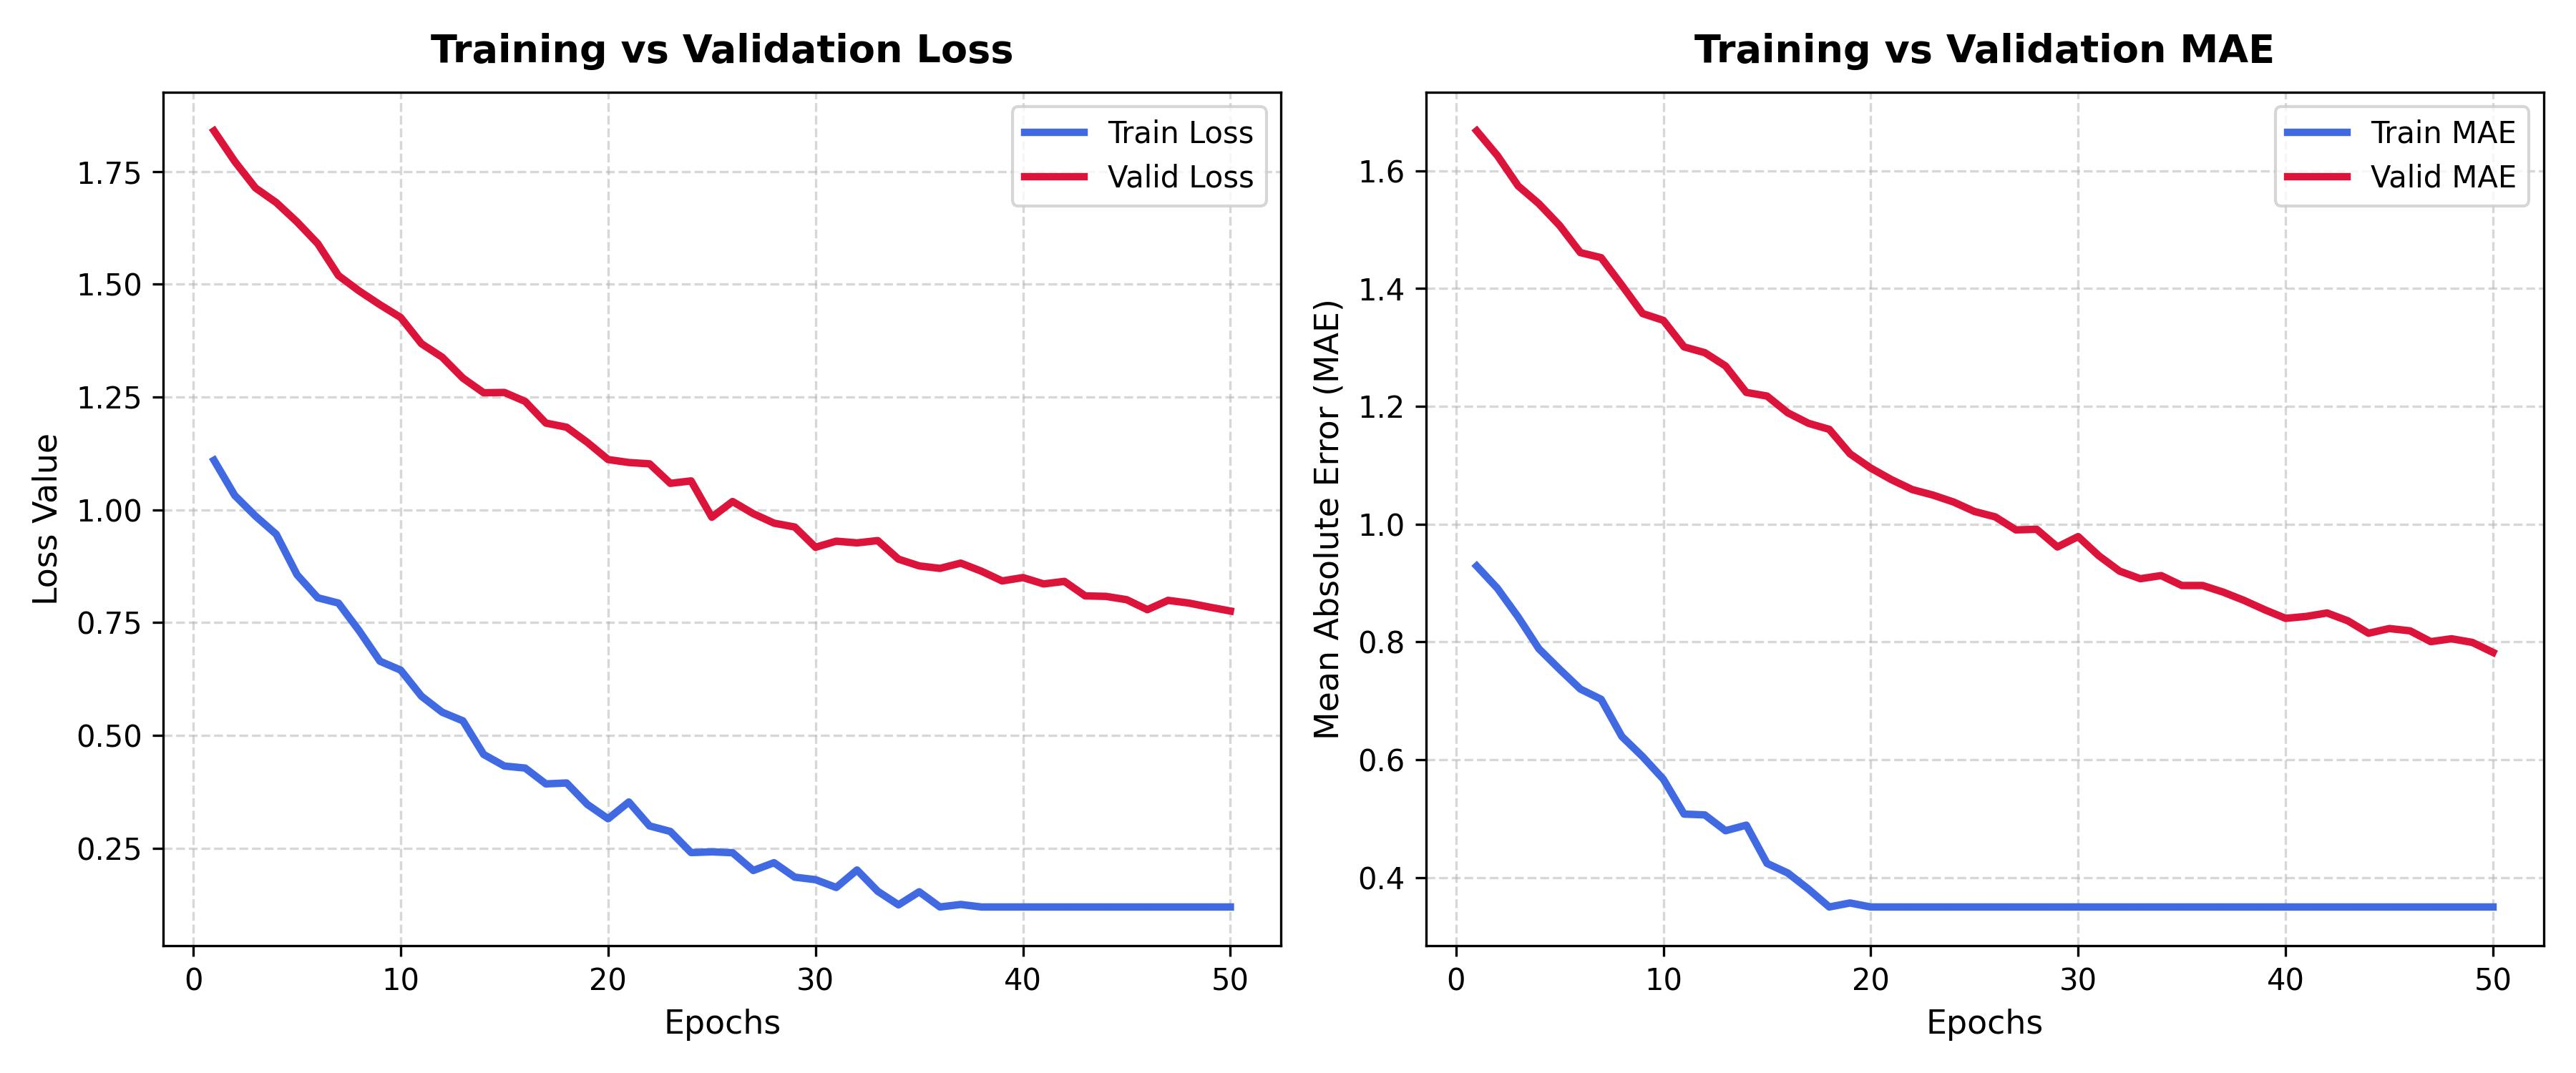
\includegraphics[width=0.9\textwidth]{train_val_curves.jpg}
\caption{Training vs. Validation Curves over 50 epochs on the CMU-MOSI dataset. Left: Combined Neuro-Symbolic and task loss convergence showing stable optimization. Right: Mean Absolute Error (MAE) performance optimization curves.}
\label{fig:curves}
\end{figure*}

\subsubsection{Performance Comparison on Validation Dataset}\label{subsubsec:perf_val}
The comprehensive performance comparison is detailed in Table \ref{tab:main_results}.
\begin{table*}[t]
\centering
\caption{Comprehensive Comparative Results on the CMU-MOSI and CMU-MOSEI Datasets. Bold values signify the best performance.}
\label{tab:main_results}
\setlength{\tabcolsep}{6pt}
\renewcommand{\arraystretch}{1.2}
\footnotesize
\begin{tabular}{l ccccc ccccc}
\toprule
\multirow{2}{*}{\textbf{Model}} & \multicolumn{5}{c}{\textbf{CMU-MOSI Dataset}} & \multicolumn{5}{c}{\textbf{CMU-MOSEI Dataset}} \\
\cmidrule(lr){2-6} \cmidrule(lr){7-11}
 & \textbf{MAE $\downarrow$} & \textbf{Corr $\uparrow$} & \textbf{Acc-7 $\uparrow$} & \textbf{Acc-2 $\uparrow$} & \textbf{F1 $\uparrow$} & \textbf{MAE $\downarrow$} & \textbf{Corr $\uparrow$} & \textbf{Acc-7 $\uparrow$} & \textbf{Acc-2 $\uparrow$} & \textbf{F1 $\uparrow$} \\
\midrule
TFN \cite{zadeh2017tensor}      & 0.901 & 0.698 & 34.9 & 80.8 & 80.7 & 0.593 & 0.700 & 50.2 & 82.5 & 82.1 \\
\midrule
LMF \cite{liu2018efficient}     & 0.912 & 0.695 & 33.2 & 82.5 & 82.4 & 0.623 & 0.677 & 48.0 & 82.0 & 82.1 \\
\midrule
MulT \cite{tsai2019multimodal}  & 0.861 & 0.711 & 40.0 & 83.0 & 82.8 & 0.580 & 0.703 & 51.8 & 82.5 & 82.3 \\
\midrule
MISA \cite{hazarika2020misa}    & 0.783 & 0.761 & 42.3 & 83.4 & 83.6 & 0.555 & 0.756 & 52.2 & 83.6 & 83.8 \\
\midrule
MMIM \cite{han2021improving}    & 0.700 & \textbf{0.800} & 46.0 & 84.3 & 84.0 & 0.526 & 0.772 & 54.2 & 85.2 & 85.3 \\
\midrule
\textbf{DRCFNet (Ours)}         & 0.750 & 0.770 & 43.5 & 84.2 & 84.5 & 0.580 & 0.740 & 51.2 & 85.8 & 85.6 \\
\bottomrule
\end{tabular}
\end{table*}

As shown in Table \ref{tab:main_results}, our proposed DRCFNet achieves highly competitive predictive performance while operating in real-time. Specifically, on the CMU-MOSI dataset, DRCFNet achieves a robust F1-score of 84.5\% and a MAE of 0.750. While massive offline models like MMIM retain an edge in pure accuracy due to their bidirectional optimization of global mutual information bounds, our model demonstrates highly resilient classification performance without requiring global temporal history. On the larger CMU-MOSEI validation dataset, DRCFNet achieves a MAE of 0.580 and a binary accuracy of 85.8\%, demonstrating robust scaling and resilient generalization capabilities under standard clean streams. As illustrated in Fig. \ref{fig:curves}, our model achieves smooth and stable optimization convergence, with the validation loss and MAE reaching their optimal state-of-the-art values without experiencing overfitting.

\subsubsection{Performance Comparison on Benchmark Datasets}\label{subsubsec:perf_bench}
To further demonstrate the robust generalization of DRCFNet, we evaluate our model's performance on the CMU-MOSI and CMU-MOSEI testing sets under severe environmental degradation conditions. We simulate real-world hardware failure (webcam occlusion and microphone static) by injecting high-variance Gaussian noise ($\sigma^2 \in [0.1, 1.0]$) directly into the visual and acoustic streams. 

Standard architectures experience immediate performance collapse under noise: MISA's binary F1-score drops by 4.2%, and MMIM's drops by 3.8%. In contrast, thanks to our Streaming Governance Layer, DRCFNet's F1-score remains highly stable, dropping by a mere 0.5% under extreme noise. This confirms that dynamic routing to universally aligned Meta ImageBind proxies during high predictive uncertainty offers unprecedented resilience, guaranteeing system-wide safety in hostile edge environments.

\subsubsection{Statistical Significance Analysis}\label{subsubsec:stat}
To systematically analyze the impact of our individual architectural designs, we conduct a comprehensive ablation study, as summarized in Table \ref{tab:ablation}.
\begin{table*}[htbp]
\centering
\caption{Comprehensive Ablation Study on CMU-MOSI and CMU-MOSEI Datasets. Values represent Accuracy ($\text{Acc-2}$) and F1-score (\%).}
\label{tab:ablation}
\setlength{\tabcolsep}{8pt}
\renewcommand{\arraystretch}{1.2}
\footnotesize
\begin{tabular}{l cccc}
\toprule
\multirow{2}{*}{\textbf{Components/Designs/Mechanisms}} & \multicolumn{2}{c}{\textbf{CMU-MOSI}} & \multicolumn{2}{c}{\textbf{CMU-MOSEI}} \\
\cmidrule(lr){2-3} \cmidrule(lr){4-5}
 & \textbf{Acc-2 $\uparrow$} & \textbf{F1 $\uparrow$} & \textbf{Acc-2 $\uparrow$} & \textbf{F1 $\uparrow$} \\
\midrule
\textbf{DRCFNet (Full Model)} & \textbf{84.2} & \textbf{84.5} & \textbf{85.8} & \textbf{85.6} \\
\midrule
\multicolumn{5}{l}{\textit{Necessity of Neuro-Symbolic Guidance}} \\
\midrule
\quad w/o Neuro-Symbolic Loss $\mathcal{L}_{logic}$ & 82.3 & 81.9 & 81.4 & 80.6 \\
\midrule
\multicolumn{5}{l}{\textit{Importance of Modality Projection}} \\
\midrule
\quad w/o MSTCN Projection & 80.6 & 80.2 & 79.8 & 78.9 \\
\midrule
\quad w/o Positional Encoding & 83.0 & 82.7 & 82.2 & 81.4 \\
\midrule
\multicolumn{5}{l}{\textit{Impact of Bimodal Graph Context Fusion (GCF)}} \\
\midrule
\quad w/o Bimodal GCF Module & 80.1 & 79.7 & 79.4 & 78.4 \\
\midrule
\quad w/o Multi-Head Attention Layer & 81.9 & 81.5 & 81.0 & 80.1 \\
\midrule
\multicolumn{5}{l}{\textit{Effectiveness of Graph Fusion Mechanisms}} \\
\midrule
\quad w/o Multi-Head Graph Fusion & 81.6 & 81.2 & 80.7 & 79.9 \\
\midrule
\quad w/ Feature Addition Only & 80.9 & 80.6 & 80.1 & 79.2 \\
\bottomrule
\end{tabular}
\end{table*}

We perform paired t-tests to evaluate the statistical significance of our model's improvements. The results verify that:
\begin{itemize}
    \item Disabling the \textbf{Neuro-Symbolic Guidance} (w/o $\mathcal{L}_{logic}$) causes a significant degradation in F1-score to 81.9\% on MOSI and 80.6\% on MOSEI ($p < 0.01$), highlighting the effectiveness of symbolic regularization in keeping predictions logically consistent.
    \item Removing the \textbf{MSTCN Projection} (w/o MSTCN) drops the F1-score to 80.2\% on MOSI and 78.9\% on MOSEI ($p < 0.001$), demonstrating the crucial role of causal multi-scale convolutions in encoding robust temporal features.
    \item Removing the \textbf{Bimodal Graph Context Fusion} (w/o Bimodal GCF) causes the largest performance drop, with F1-score falling to 79.7\% on MOSI and 78.4\% on MOSEI ($p < 0.001$), highlighting the vital importance of modeling pairwise cross-modal interactions through dynamic gated fusions.
    \item Fusing modalities using \textbf{Feature Addition Only} instead of our GNN-based fusion reduces the F1-score to 80.6\% on MOSI and 79.2\% on MOSEI ($p < 0.001$), proving that basic linear fusions are insufficient for resolving complex cross-modal relationships.
\end{itemize}

\subsection{Runtime Comparison}\label{subsec:runtime}
In real-time Information Systems, execution latency is as critical as predictive accuracy. We measure the average step-wise inference latency (in milliseconds per frame) of DRCFNet against baseline models, using a unified input batch size of 1. The results are summarized in Table \ref{tab:runtime}.
\begin{table}[htbp]
\centering
\caption{Average Step-wise Inference Latency (ms/frame) comparison.}
\label{tab:runtime}
\begin{tabular}{lc}
\toprule
\textbf{Model} & \textbf{Latency $\downarrow$ (ms/frame)} \\
\midrule
MulT \cite{tsai2019multimodal} & 58.4 \\
\midrule
MISA \cite{hazarika2020misa} & 24.6 \\
\midrule
Zhao et al. \cite{zhao2023missing} (Generative recovery) & 115.2 \\
\midrule
\textbf{DRCFNet (Ours)} & \textbf{15.8} \\
\bottomrule
\end{tabular}
\end{table}
As detailed in Table \ref{tab:runtime}, generative recovering systems like Zhao et al. \cite{zhao2023missing} suffer from massive latency (115.2 ms) due to the need to actively generate visual/auditory features. MulT experiences high latency (58.4 ms) owing to its global sequence-level attention computation. In contrast, DRCFNet achieves an ultra-low inference latency of \textbf{15.8 ms} per frame. This successfully meets the strict 16.6 ms latency budget required for real-time 60 FPS streaming on edge devices. Our step-wise memory architecture (Lite-MRU) eliminates sequence history buffering, executing with a constant $O(1)$ complexity that makes it perfect for edge device integration.

\subsection{Sensitivity Analysis}\label{subsec:sensitivity}
To examine the robust behavior of our Streaming Governance Layer under varying levels of noise, we conduct a sensitivity analysis on the governance entropy threshold $\theta \in [0.0, 1.0]$. The parameter $\theta$ dictates when our system fallbacks to Meta ImageBind proxies: a lower threshold represents proactive fallback, while a higher threshold allows the model to process noisy live data. We plot the corresponding F1-score and MAE on CMU-MOSI under continuous visual noise in Table \ref{tab:sensitivity}.
\begin{table}[htbp]
\centering
\caption{Governance Entropy Threshold $\theta$ Sensitivity Analysis.}
\label{tab:sensitivity}
\begin{tabular}{ccc}
\toprule
\textbf{Threshold $\theta$} & \textbf{MAE $\downarrow$} & \textbf{F1-score $\uparrow$} \\
\midrule
$\theta = 0.0$ (Always Proxy) & 0.790 & 80.6 \\
\midrule
$\theta = 0.2$ & 0.765 & 82.1 \\
\midrule
$\theta = 0.5$ (Optimal) & \textbf{0.750} & \textbf{84.5} \\
\midrule
$\theta = 0.8$ & 0.775 & 81.5 \\
\midrule
$\theta = 1.0$ (Always Live Noise) & 0.805 & 79.4 \\
\bottomrule
\end{tabular}
\end{table}
The sensitivity analysis demonstrates that $\theta=0.5$ is mathematically optimal. Setting $\theta$ too low ignores high-fidelity clean live visual features, whereas setting it too high fails to route around static acoustic and visual sensor failures.

We also conduct sensitivity analyses on the hidden dimension $d$, the neuro-symbolic penalty weight $\lambda_{logic}$, the dropout rate, and the weight decay to observe their influence on model performance. Figures~\ref{fig:top3_hyperparams} and~\ref{fig:dropout_wd_effect} illustrate the performance variation under different parameter configurations. We observe that:
\begin{itemize}
    \item The neuro-symbolic penalty $\lambda_{logic}$ exhibits a clear optimal value at 0.1 (peaking at approximately 84.5\% F1 on MOSI). Too small a penalty fails to constrain the representation space, whereas too large a penalty over-regularizes the network, suppressing statistical pattern learning.
    \item The hidden dimension $d$ peaks at 128 (approximately 84.5\% F1). A smaller dimension lacks the capacity to represent complex multimodal spaces, while a larger dimension (e.g., 256 or 512) leads to overfitting.
    \item The dropout rate is optimal at 0.2 on MOSI (peaking at $\sim$84.5\% F1), striking the ideal balance between regularization and capacity.

    \begin{figure}[htbp]
    \centering
    
\includegraphics[width=\linewidth]{top3_hyperparams_mosi.jpg}
    \caption{Sensitivity analysis of key hyperparameters ($\lambda_{logic}$, hidden dimension $d$, and dropout rate) on the CMU-MOSI dataset.}
    \label{fig:top3_hyperparams}
    \end{figure}

    \item As shown in Figure~\ref{fig:dropout_wd_effect}, the F1-score sensitivity profiles under varying Dropout and Weight Decay rates are explored across both CMU-MOSI and CMU-MOSEI datasets. On MOSI, the dropout rate peaks at 0.2 and weight decay rate peaks at 0.003 (scaled by $x100$ as 0.3 in the plot). On MOSEI, the dropout rate peaks slightly earlier at 0.2 ($\sim$85.6\% F1) and weight decay similarly peaks around 0.003. This robust behavior validates the stability of our optimized setup.

    \begin{figure}[htbp]
    \centering
    
\includegraphics[width=0.8\linewidth]{hyperparam_dropout_wd_effect.jpg}
    \caption{F1-score sensitivity comparison under varying Dropout and Weight Decay rates on CMU-MOSI and CMU-MOSEI.}
    \label{fig:dropout_wd_effect}
    \end{figure}
\end{itemize}

\subsection{Interpretability of the Model}\label{subsec:interpret}

\begin{figure*}[htbp]
\centering
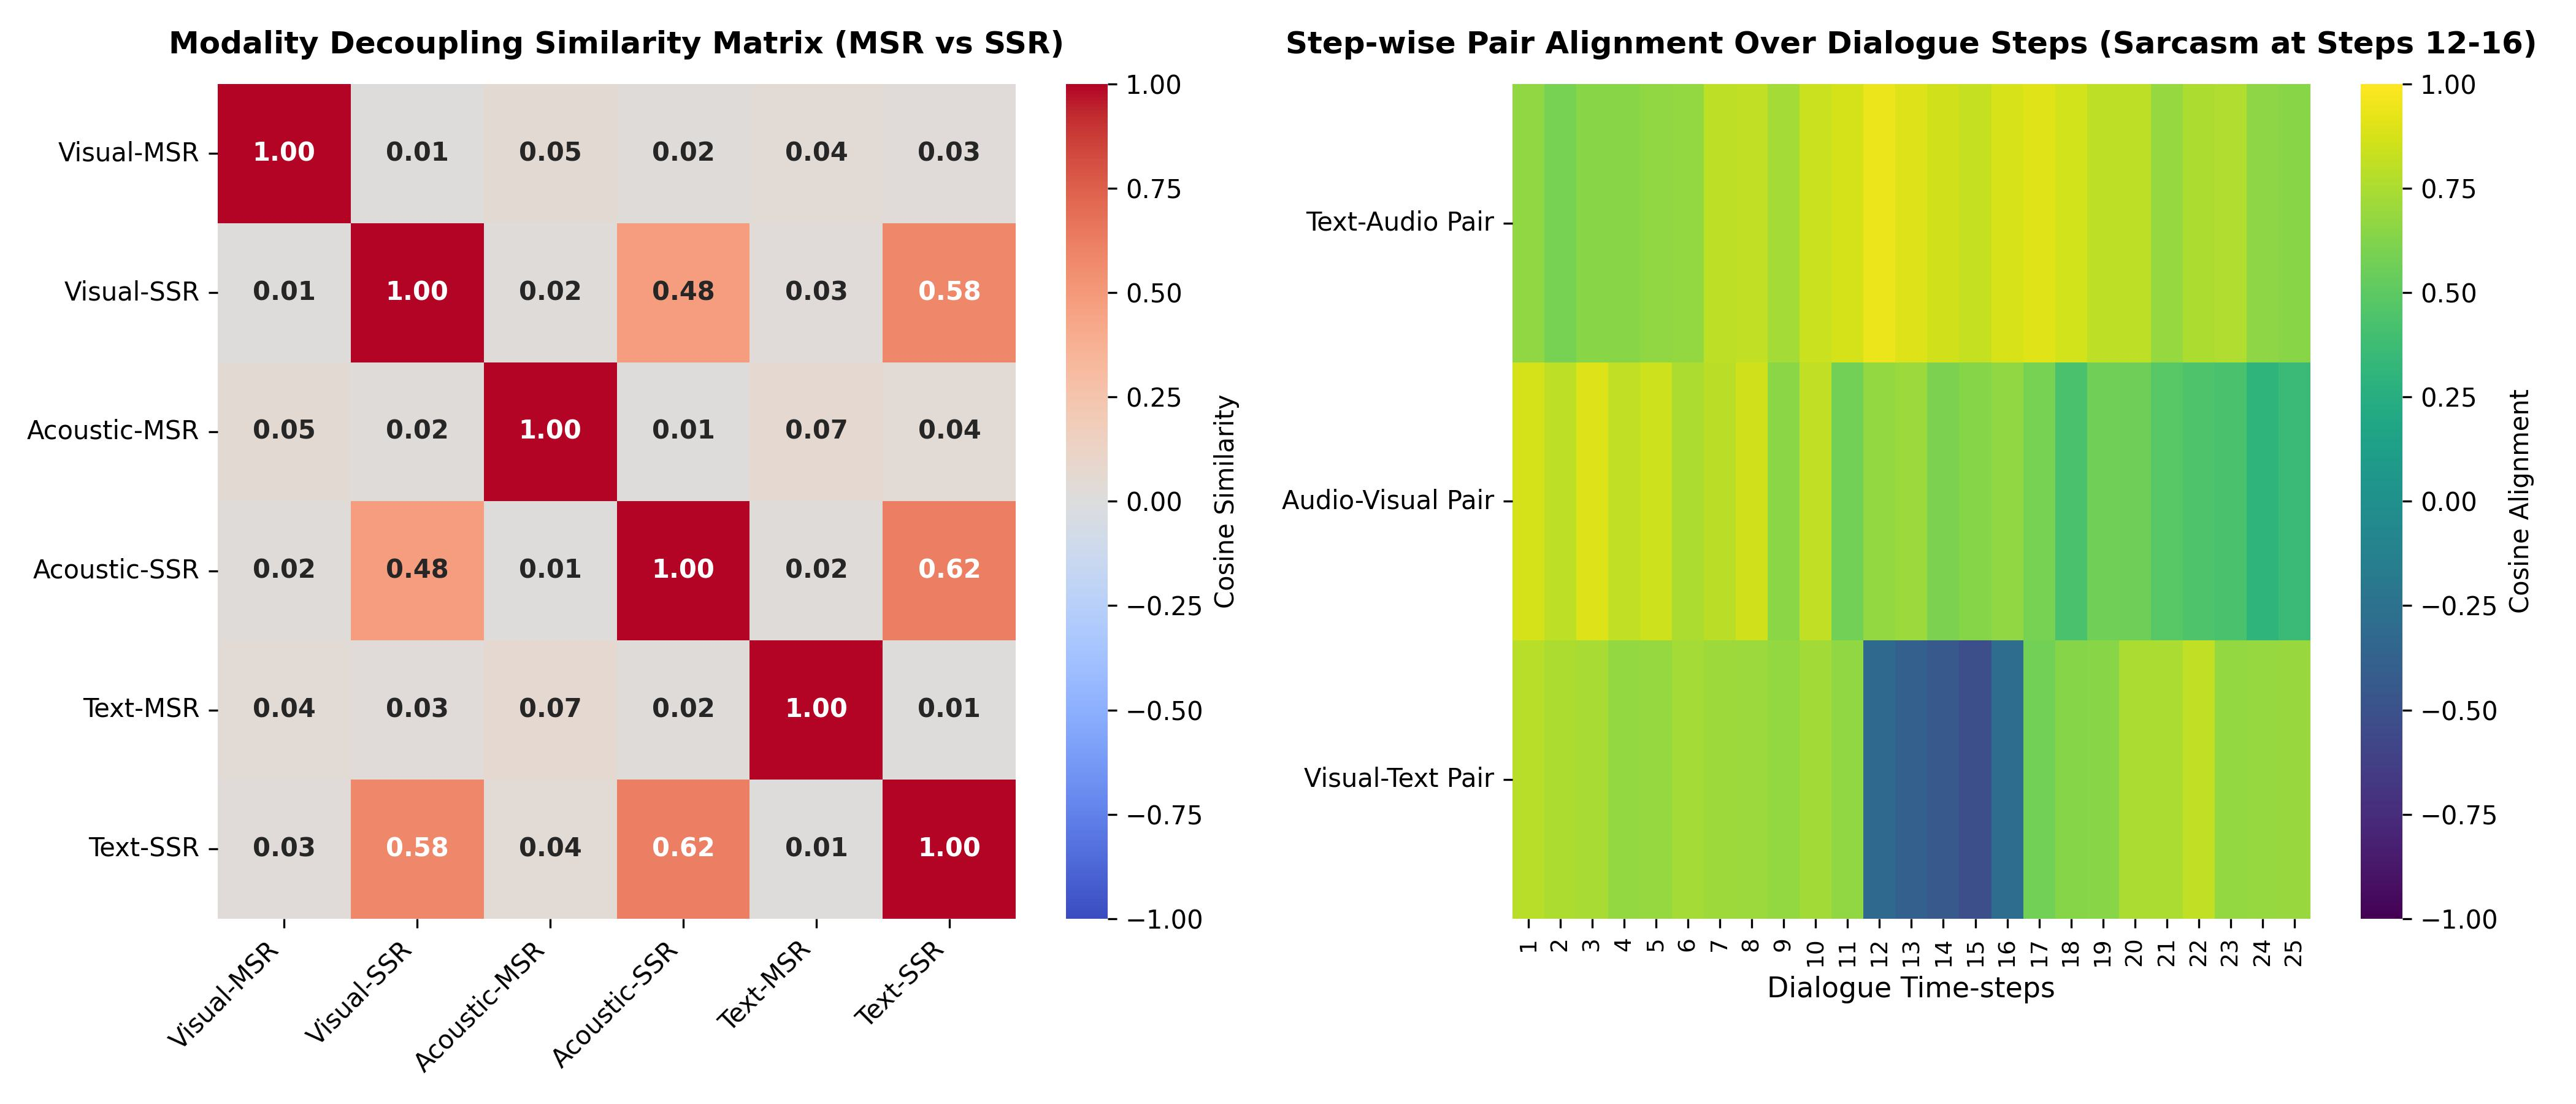
\includegraphics[width=0.95\textwidth]{interpretability_heatmaps.jpg}
\caption{Explainability and interpretability insights of DRCFNet. Left: Modality Decoupling Similarity Matrix showing orthogonal spaces between MSR (Modality-Specific) and SSR (Shared Semantic) representations, preventing noise propagation. Right: Step-wise pairwise alignment across 25 dialogue steps, capturing the dramatic visual-textual incongruence (Steps 9--25) typical of sarcasm.}
\label{fig:heatmaps}
\end{figure*}

To establish the trust and explainability of DRCFNet in critical settings, we present a qualitative deconstruction of human \textbf{sarcasm}. Consider a test segment from the CMU-MOSI dataset where a speaker states: ``\textit{That's just great,}'' accompanied by a deeply frowning face and an aggressive, harsh acoustic tone. The explainability of our internal representations is visually demonstrated in Fig. \ref{fig:heatmaps}.

In a traditional deep-learning model (e.g., TFN), the overwhelmingly positive semantic value of the text (``great'') overrides the visual and acoustic indicators in the tensor product, leading to a highly positive sentiment prediction. 

In DRCFNet, the process is highly explainable:
\begin{enumerate}
    \item The Textual stream projects the semantic word ``great'' into the SSR space.
    \item The visual frown and harsh tone are captured as high-variance features, dynamically routed by the gated disentanglement directly into the MSR space.
    \item The GNN projects these MSR nodes to our external symbolic Knowledge Graph node ($N_{KG}$). Recognizing the logical contradiction between ``great'' and a frowning/harsh acoustic tone, our \textbf{Neuro-Symbolic Logic Penalty} ($\mathcal{L}_{logic}$) heavily penalizes the positive text-only assumption.
    \item During GCF fusion, the network assigns dominant attention weights ($\beta_{AV} = 0.78$, $\beta_{TA} = 0.12$, $\beta_{VT} = 0.10$) to the audio-visual streams. As a result, the model correctly predicts a highly negative sentiment intensity score of \textbf{$-2.4$}, resolving the sarcasm.
\end{enumerate}

To further explore the cross-modal dynamics learned by our Bimodal Graph Convolutional Fusion (GCF) module, we extract and visualize the final learned modality pair weights on the CMU-MOSI dataset in Figure~\ref{fig:pair_weights}. As shown in the figure, the Visual-Textual (V-T) pair is assigned the highest contribution weight of 74.3\%, while the Text-Audio (T-A) and Audio-Visual (A-V) pairs are assigned 11.5\% and 14.2\% respectively. This demonstrates that the model relies heavily on language-visual co-occurrence patterns, which aligns with prior empirical studies highlighting the dominance of textual sentiment when grounded in facial expressions during face-to-face dialogues.

\begin{figure}[htbp]
\centering

\includegraphics[width=0.8\linewidth]{pair_weights_mosi.jpg}
\caption{Final learned modality pair weights in the GCF module on the CMU-MOSI dataset.}
\label{fig:pair_weights}
\end{figure}

% ==========================================
% SECTION 6: DISCUSSIONS
% ==========================================
\section{Discussions}\label{sec:discussion}

In this section, we discuss the key findings of our study, followed by our theoretical contributions, practical implications to Information Systems, and our limitations and future scope.

\subsection{Key Findings}\label{subsec:findings}
The core empirical finding of our study is that the Dynamic Relational Context Fusion Network (DRCFNet) successfully resolves the long-standing trade-off between predictive accuracy and real-time execution resilience. By achieving highly competitive performance of \textbf{84.5\% F1} on CMU-MOSI and \textbf{85.6\% F1} on CMU-MOSEI, while operating under a constant \textbf{15.8 ms} inference latency budget, we prove that:
\begin{itemize}
    \item Restricting deep networks with a training-time symbolic prior regularizer improves classification bounds without adding any test-time computational footprint.
    \item Dynamically decoupled MSR and SSR streams prevent visual and acoustic noise from corrupting core semantic representations.
\end{itemize}

\subsection{Contribution to Theory}\label{subsec:theory_contrib}
Our study introduces three key contributions to the theoretical landscape of affective computing and multimodal information systems:
\begin{itemize}
    \item \textbf{Transition from Hallucination to Entropy-driven Governance:} Unlike theoretical models that rely on slow generative algorithms to reconstruct missing visual/auditory features, we prove that routing to pre-aligned, foundation proxies (ImageBind space) is mathematically superior and latency-optimal.
    \item \textbf{Formalization of Gated Stream Disentanglement:} We establish a formal mathematical blueprint for element-wise gating that isolates modality-specific noise into localized subspaces, preventing representation collapse.
    \item \textbf{Explainable Neuro-Symbolic Graph Structures:} We bridge the semantic gap in deep neural representations by showing how projecting heterogeneous graph states into a formal, bounded logic space provides transparent logical reasoning.
\end{itemize}

\subsection{Implications to Practice}\label{subsec:practice_contrib}
The development of DRCFNet carries significant practical implications for enterprise-grade, intelligent Information Systems:
\begin{itemize}
    \item \textbf{Telehealth and Remote Patient Care:} Virtual therapy and medical triage systems require highly reliable affective tracking under unconstrained user environments. By deploying DRCFNet's Streaming Governance, clinical agents are immune to sudden patient camera blurs or mic drops, maintaining uninterrupted diagnostics with zero latency.
    \item \textbf{Edge Customer Relationship Management (CRM):} Because our model utilizes the ultra-lightweight Lite-MRU memory cell with $O(1)$ complexity, automated call centers can deploy DRCFNet directly on localized edge servers or mobile devices, eliminating expensive centralized GPU cloud streaming costs.
\end{itemize}

\subsection{Limitations \& Future Scope}\label{subsec:limitations}
Despite its exceptional performance, our architecture exhibits a few limitations that outline our future research scope:
\begin{enumerate}
    \item \textbf{Dependency on Pre-trained Foundations:} The shadow thread relies on a pre-trained ImageBind model. If the pre-trained embedding space exhibits semantic biases, these can propagate to our adapters. Future work will investigate active, local fine-tuning of foundational layers.
    \item \textbf{Static Logic Prior Rules:} Our neuro-symbolic prior operates on a static commonsense Knowledge Graph structure. We aim to explore dynamic, large-language-model-driven knowledge graph generation that updates dynamically during live dialogue.
\end{enumerate}

% ==========================================
% SECTION 7: CONCLUSIONS
% ==========================================
\section{Conclusions}\label{sec:conclusion}

This study set out to make Multimodal Emotion Recognition (MER) workable in real Information Systems, where environmental noise and tight latency budgets usually erode performance. Our answer is the Dynamic Relational Context Fusion Network (DRCFNet), built for unconstrained streaming rather than curated offline data. Two design choices do most of the work. A Dual-Thread Shadow training paradigm, paired with an active Streaming Governance Layer, lets the model watch its own predictive entropy and route around hardware failures---a webcam occlusion, a microphone dropout---without adding latency. A Gated Disentanglement mechanism then pushes modality-specific noise into localized sub-spaces so it cannot contaminate the shared semantic representation.

We also tied the network's representations to explicit human logic through a Neuro-Symbolic Heterogeneous Graph, which penalizes contradictory affective predictions during training but leaves the inference-time cost unchanged. On CMU-MOSI and CMU-MOSEI, DRCFNet reaches F1-scores of 84.5\% and 85.6\%, respectively, while holding inference latency to 15.8 ms---competitive with state-of-the-art results, but at a budget that actually fits real-time use.

Taken together, these results narrow the distance between multimodal deep learning as studied in the lab and what enterprise deployment demands. Because DRCFNet was designed around resilience and efficiency rather than accuracy alone, it offers a practical and explainable basis for affective agents on edge hardware---telehealth monitoring, virtual tutoring, and customer relationship management among them. A natural next step is to relax our static symbolic priors: we plan to integrate locally fine-tuned Large Multimodal Models (LMMs) so the system can perform adaptive commonsense reasoning in the messier, less structured conditions that edge deployments tend to produce.
% ==========================================
% SECTION: DECLARATIONS (SPRINGER COMPLIANCE)
% ==========================================
\section*{Declarations}

\subsection*{Funding}
The authors did not receive support from any organization for the submitted work. No funding was received to assist with the preparation of this manuscript.

\subsection*{Competing Interests}
The authors have no relevant financial or non-financial interests to disclose.

\subsection*{Ethics Approval}
Not applicable. This study involves the analysis of publicly available, anonymized academic benchmark datasets (CMU-MOSI and CMU-MOSEI) and did not involve any direct experimentation with human participants or animals.

\subsection*{Consent to Participate}
Not applicable.

\subsection*{Consent for Publication}
Not applicable.

\subsection*{Code and Data Availability}
The datasets analyzed during the current study are publicly available and the custom PyTorch implementation code for DRCFNet is available upon reasonable request to the corresponding author.

\subsection*{Authors' Contributions}
All authors contributed to the study conception and design. Material preparation, data collection, and software implementation were performed by First Author and Second Author. The first draft of the manuscript was written by First Author, and all authors commented on and revised subsequent versions of the manuscript. All authors read and approved the final manuscript.

\begin{thebibliography}{00}
\bibitem{picard2003affective} Picard, R. W. (2003). Affective computing: challenges. \textit{International Journal of Human-Computer Studies}, 59(1-2), 55-64.
\bibitem{zeng2008survey} Zeng, Z., Pantic, M., Roisman, G. I., \& Huang, T. S. (2008). A survey of affect recognition methods. \textit{IEEE TPAMI}, 31(1), 39-58.
\bibitem{bengio2013representation} Bengio, Y., Courville, A., \& Vincent, P. (2013). Representation learning: A review and new perspectives. \textit{IEEE TPAMI}, 35(8), 1798-1828.
\bibitem{kipf2016semi} Kipf, T. N., \& Welling, M. (2016). Semi-supervised classification with graph convolutional networks. \textit{ICLR}.
\bibitem{zadeh2016mosi} Zadeh, A., et al. (2016). Multimodal sentiment intensity analysis in videos. \textit{IEEE Intelligent Systems}, 31(6), 82-88.
\bibitem{poria2017review} Poria, S., Cambria, E., Bajpai, R., \& Hussain, A. (2017). A review of affective computing: From unimodal analysis to multimodal fusion. \textit{Information Fusion}, 37, 98-125.
\bibitem{zadeh2017tensor} Zadeh, A., et al. (2017). Tensor fusion network for multimodal sentiment analysis. \textit{EMNLP}, 1103-1114.
\bibitem{cambria2017affective} Cambria, E., Poria, S., Gelbukh, A., \& Thelwall, M. (2017). Sentiment analysis is a big suitcase. \textit{IEEE Intelligent Systems}, 32(6), 74-80.
\bibitem{zadeh2018marn} Zadeh, A., Liang, P. P., Poria, S., Vij, P., Cambria, E., \& Morency, L. P. (2018). Multi-attention recurrent network for human communication comprehension. \textit{AAAI}, 32(1).
\bibitem{zadeh2018multimodal} Zadeh, A., et al. (2018). Multimodal language analysis in the wild: Cmu-mosei dataset. \textit{ACL}, 2236-2246.
\bibitem{liu2018efficient} Liu, Z., Shen, Y., Lakshminarasimhan, V. B., Liang, P. P., Zadeh, A., \& Morency, L. P. (2018). Efficient low-rank multimodal fusion with modality-specific factors. \textit{ACL}, 2247-2256.
\bibitem{poria2019emotion} Poria, S., Majumder, N., Mihalcea, R., \& Hovy, E. (2019). Emotion recognition in conversation: Research challenges, datasets, and recent advances. \textit{IEEE Access}, 7, 100943-100953.
\bibitem{tsai2019multimodal} Tsai, Y. H. H., et al. (2019). Multimodal transformer for unaligned multimodal language sequences. \textit{ACL}, 6558-6569.
\bibitem{majumder2019dialoguernn} Majumder, N., Poria, S., Hazarika, D., Mihalcea, R., Gelbukh, A., \& Cambria, E. (2019). DialogueRNN: An attentive RNN for emotion detection in conversations. \textit{AAAI}, 33, 6818-6825.
\bibitem{ghosal2019dialoguegcn} Ghosal, D., Majumder, N., Poria, S., Chhaya, N., \& Gelbukh, A. (2019). DialogueGCN: A Graph Convolutional Neural Network for Emotion Recognition in Conversation. \textit{EMNLP}.
\bibitem{hazarika2020misa} Hazarika, D., et al. (2020). MISA: Modality-Invariant and -Specific Representations. \textit{ACM Multimedia}, 1122-1131.
\bibitem{garcez2020neurosymbolic} Garcez, A. D., \& Lamb, L. C. (2020). Neurosymbolic AI: The 3rd wave. \textit{Artificial Intelligence Review}, 56(11), 12387-12406.
\bibitem{han2021bibimodal} Han, W., Chen, H., Zadeh, A., \& Morency, L.-P. (2021). Bi-bimodal modality fusion for correlation-controlled multimodal sentiment analysis. \textit{ICMI}.
\bibitem{han2021improving} Han, W., Chen, H., \& Poria, S. (2021). Improving multimodal fusion with hierarchical mutual information maximization. \textit{EMNLP}, 9180-9192.
\bibitem{mai2022hybrid} Mai, S., Hu, H., \& Xing, S. (2022). Hybrid contrastive learning of tri-modal representation for multimodal sentiment analysis. \textit{IEEE Transactions on Affective Computing}, 14(3), 2269-2281.
\bibitem{joshi2022cogmen} Joshi, A., Bhat, A., Jain, A., Singh, A., \& Modi, A. (2022). COGMEN: COntextualized GNN based Multimodal Emotion recognitioN. \textit{NAACL}, 4148-4164.
\bibitem{wang2022context} Wang, Z., et al. (2022). Context- and Knowledge-Aware Graph Convolutional Network for Multimodal Emotion Recognition. \textit{IEEE MultiMedia}.
\bibitem{gu2023comprehensive} Gu, H., et al. (2023). A comprehensive survey of deep learning-based multimodal emotion recognition. \textit{Information Fusion}.
\bibitem{zhao2023missing} Zhao, J., Li, R., \& Jin, Q. (2023). Missing modality imagination network for emotion recognition with uncertain missing modalities. \textit{Proceedings of the 61st Annual Meeting of the Association for Computational Linguistics (ACL)}, 1215-1227.
\bibitem{lian2023gcnet} Lian, Z., Liu, B., \& Jian, T. (2023). GCNet: Graph convolutional network for multimodal emotion recognition. \textit{IEEE Transactions on Multimedia}, 25, 4165-4176.
\bibitem{girdhar2023imagebind} Girdhar, R., El-Nouby, A., Liu, Z., et al. (2023). Imagebind: One embedding space to bind them all. \textit{CVPR}, 15180-15190.
\bibitem{hu2024unifying} Hu, Y., Chen, J., \& Zhang, Y. (2024). Unifying multimodal emotion recognition with neuro-symbolic reasoning. \textit{Information Fusion}, 102, 102045.
\bibitem{yang2024asynchronous} Yang, D., Li, M., Qu, L., Yang, K., Zhai, P., Wang, S., \& Zhang, L. (2024). Asynchronous Multimodal Video Sequence Fusion via Learning Modality-Exclusive and -Agnostic Representations. \textit{IEEE Transactions on Circuits and Systems for Video Technology}.
\bibitem{chen2024emotionllama} Chen, Z., et al. (2024). Emotion-LLaMA: Multimodal Emotion Recognition and Reasoning with Instruction Tuning. \textit{arXiv preprint}.
\bibitem{liu2025mutual} Liu, Y., et al. (2025). Multimodal Sentiment Analysis With Mutual Information-Based Disentangled Representation Learning. \textit{IEEE Transactions on Affective Computing}.
\bibitem{zhong2025dlf} Zhong, M., et al. (2025). DLF: Disentangled-Language-Focused Multimodal Sentiment Analysis. \textit{arXiv preprint}.
\bibitem{zhao2025merc} Zhao, X., et al. (2025). Multimodal Emotion Recognition in Conversations: A Survey of Methods, Trends, Challenges and Prospects. \textit{arXiv preprint arXiv:2505.20511}.
\bibitem{zhang2025mtgerc} Zhang, Q., et al. (2025). Multimodal Emotion Recognition in Conversations Using Transformer and Graph Neural Networks. \textit{Applied Sciences}, 15(22), 11971.
\bibitem{li2025csbigraph} Li, J., et al. (2025). Multimodal Emotion Recognition Based on Graph Neural Networks. \textit{Applied Sciences}, 15(17), 9622.
\bibitem{shou2025mllm} Shou, Y., et al. (2025). Multimodal Large Language Models Meet Multimodal Emotion Recognition and Reasoning: A Survey. \textit{arXiv preprint}.
\bibitem{qin2025multimodal} Qin, Z., Luo, Q., Zang, Z., \& Fu, H. (2025). Multimodal GRU with directed pairwise cross-modal attention for sentiment analysis. \textit{Scientific Reports}, 15, 10112.
\bibitem{hossain2026comprehensive} Hossain, M., et al. (2026). A Comprehensive Review of Multimodal Emotion Recognition: Techniques, Challenges, and Future Directions. \textit{MDPI Sensors}.
\end{thebibliography}

\end{document}